\section{The Dependence of the Beam Coupling Impedance on The Kicker Components}

As part of the study to improve the beam screen it was decided to investigate systematically the effect of the various commponents of the kicker magnet on the resulting beam coupling impedance. This is divided into two sections, the study of the effect of the beam screen on the beam coupling impedance of the ferrite yoke, and subsequently a study of the effects of the dimensions of the beam screen and screen conductors on the beam coupling impedance.

\subsection{The Impedance of the MKI - Effects of the Inclusion of the Beam Screen}

To first judge the effectiveness of the concept of the beam screen as an impedance reduction technique we simulate the MKI by systematically adding components to the magnet to determine their effect on the beam coupling impedance. We consider the following configurations of the MKI:

\begin{enumerate}
\item{The c-core ferrite yoke}
\item{The c-core ferrite yoke with a ceramic cylinder inserted inside}
\item{As above but with 24 screen conductors inserted into the cylinder, capactively coupled at one end}
\item{The internal magnet structure including the vacuum tank, HV and ground plates and the surrounding connections.}
\end{enumerate}

These geometries are shown in Fig.~\ref{fig:mki-layout-buildup}, and the resulting impedance simulations for the real component shown in Fig.~\ref{fig:mki-buildup-impedance}. Several points can be seen; firstly that the inclusion of the beam screen with screen conductors very effectively screens the beam from the other components of the kicker magnet - including the ceramic of the beam screen, the surrounding structures and the ferrite itself. This indicates that for a beam screen in which the ceramic tube holds a large number of screen conductors, the beam is effectively screened from the surrounding structure up to a frequency characterised by seperation of the screen conductors. This has benefits for the impedance simulations as it is valid to use a reduced simulation model considering just the capacitively coupled end provided we can assume the ferrite is well screened (i.e. we have 24 screen conductors in place). Secondly the inclusion of the ceramic beam pipe does not effectively screen the ferrite by itself - the screen conductors are necessary to correctly screen the surroundings. And lastly that the use of the ceramic beam screen contributes significantly to the imaginary component of the longitudinal impedance (evidenced by the linear increase of the imaginary impedance with frequency due to the inductive component of the impedance) even with the presence of screen conductors.
 
\begin{figure}
\subfigure[]{
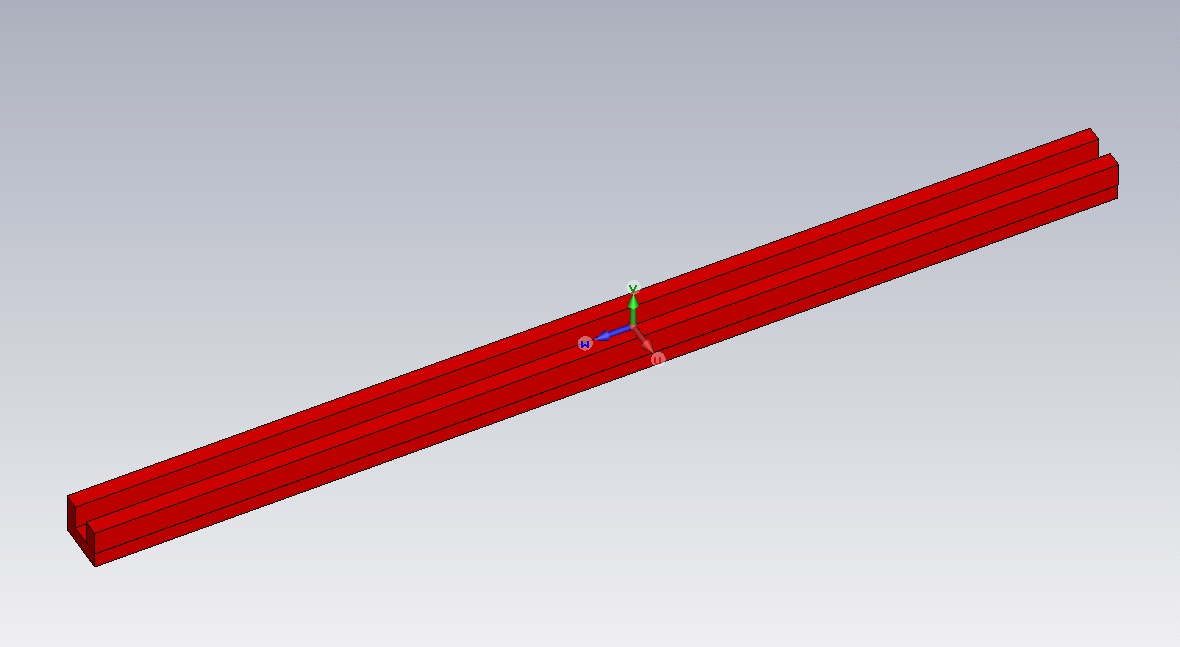
\includegraphics[width=0.45\textwidth]{LHC_MKI/figures/mki-buildup-ferrite.png}
\label{fig:mki-buildup-ferrite}
}
\subfigure[]{
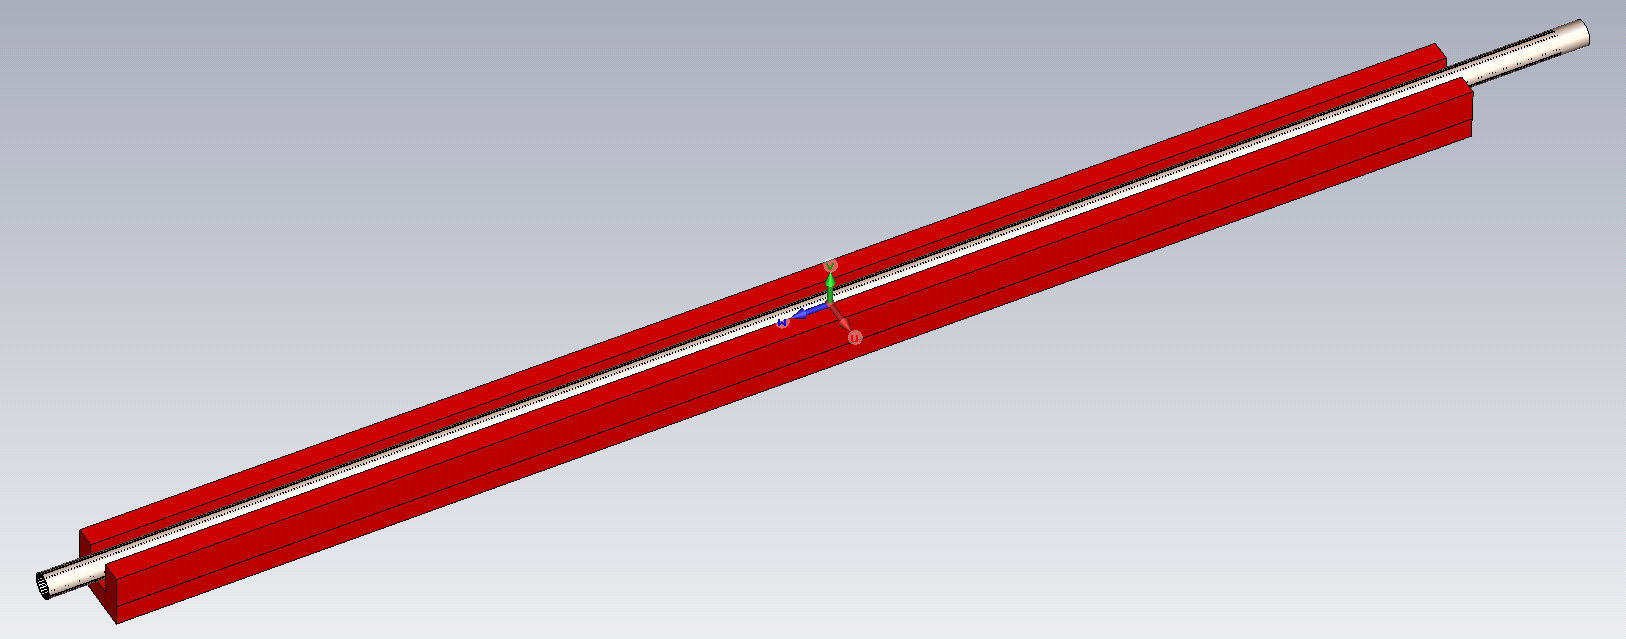
\includegraphics[width=0.45\textwidth]{LHC_MKI/figures/mki-buildup-ferrite-ceramic.png}
\label{fig:mki-buildup-ferrite-ceramic}
}
\subfigure[]{
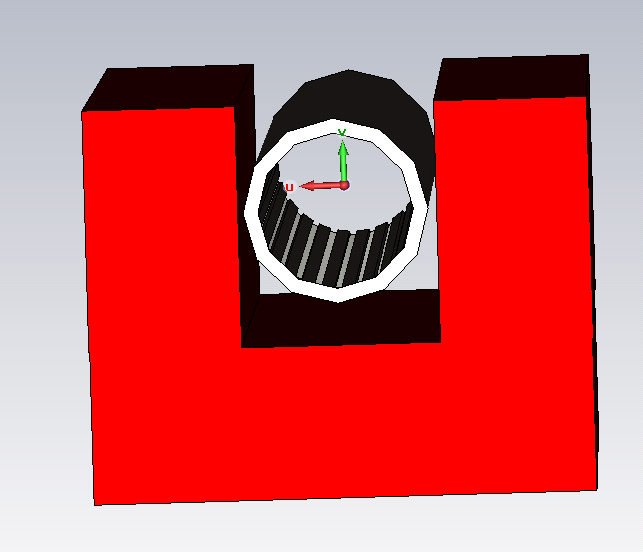
\includegraphics[width=0.45\textwidth]{LHC_MKI/figures/mki-buildup-ferrite-ceramic-cond.png}
\label{fig:mki-buildup-ferrite-ceramic-cond}
}
\subfigure[]{
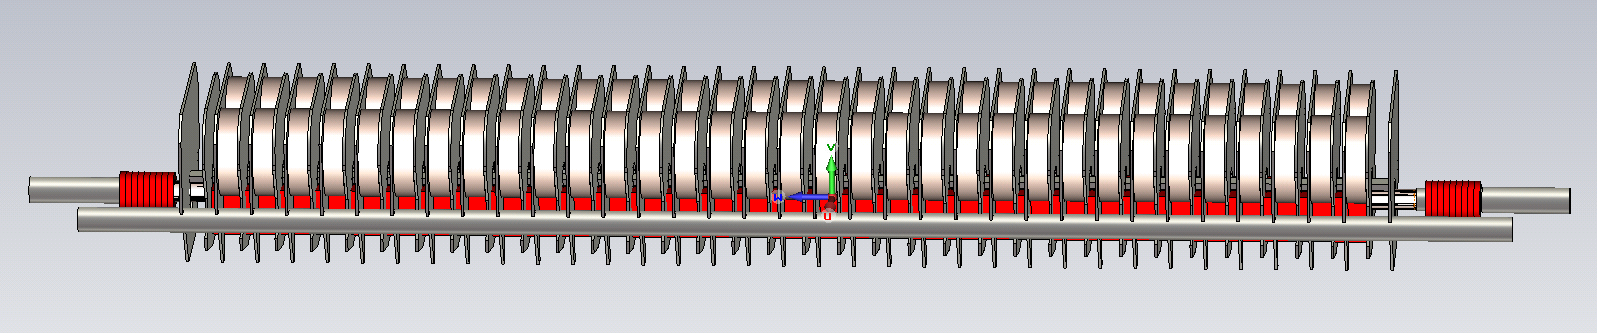
\includegraphics[width=0.45\textwidth]{LHC_MKI/figures/mki-buildup-ferrite-ceramic-cond-full.png}
\label{fig:mki-buildup-ferrite-ceramic-cond-full}
}
\label{fig:mki-layout-buildup}
\caption{The geometries simulated for the various components in the LHC-MKI. These are ferrite only \ref{fig:mki-buildup-ferrite}, ferrite and the ceramic beam screen \ref{fig:mki-buildup-ferrite-ceramic}, ferrite with the beam screen containing 24 screen conductors \ref{fig:mki-buildup-ferrite-ceramic-cond} and finally the complete MKI magnet \ref{fig:mki-buildup-ferrite-ceramic-cond-full}.}
\end{figure}

\begin{figure}
\subfigure[]{
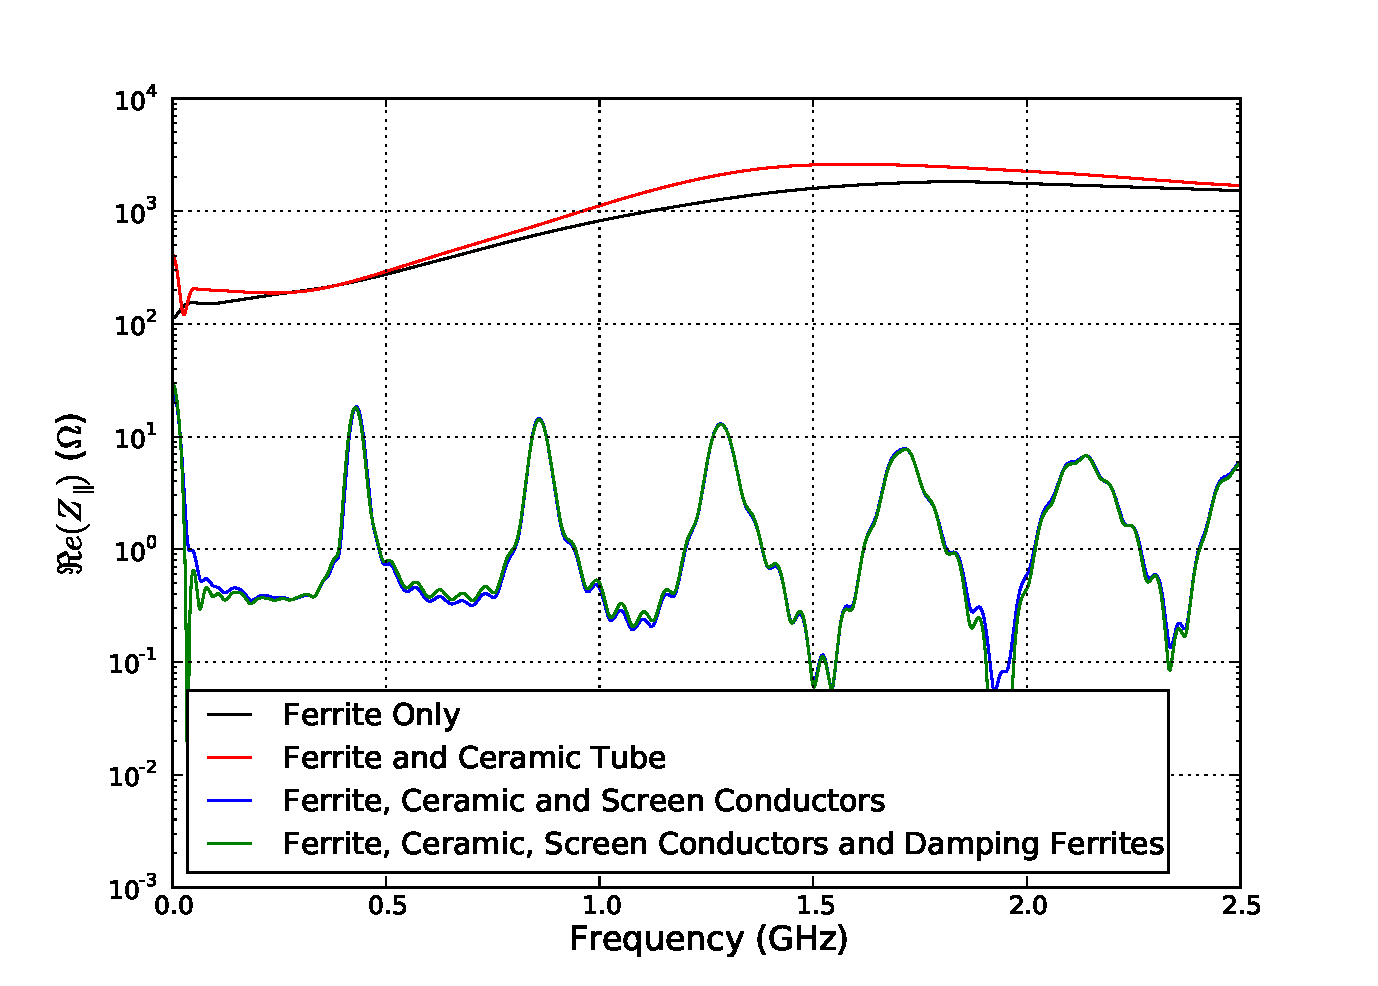
\includegraphics[width=0.5\textwidth]{LHC_MKI/figures/mki-build-up-real-imp.pdf}
\label{fig:mki-buildup-real-imp}
}
\subfigure[]{
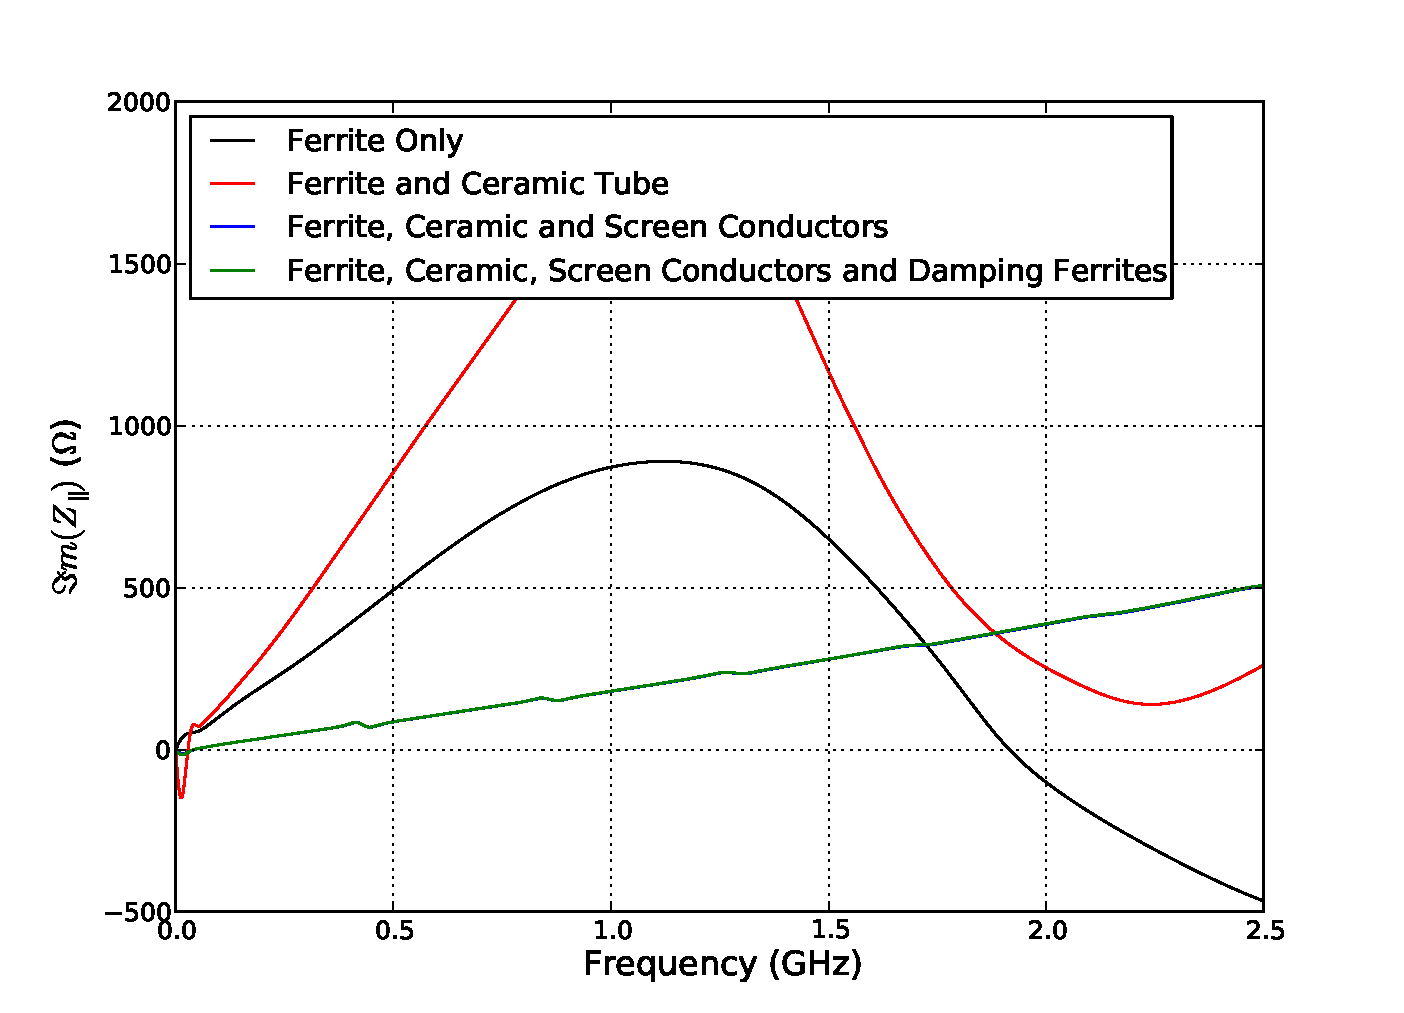
\includegraphics[width=0.5\textwidth]{LHC_MKI/figures/mki-build-up-imag-imp.pdf}
\label{fig:mki-buildup-imag-imp}
}
\label{fig:mki-buildup-impedance}
\caption{The \ref{fig:mki-buildup-real-imp} real component and the \ref{fig:mki-buildup-imag-imp} imaginary components of the LHC MKI kicker magnet impedances for different quantities of components in the magnet.}
\end{figure}

\subsection{The Role of the Beam Screen Layout in the Impedance of the MKI}

Concerning the role of the beam screen layout there are two areas to examine - the effect of different quantities of screening of the beam by having more or less screen conductors (in this case removing those directed towards the HV busbar as is likely due to concerns of electrical breakdown) and of the effect of different dimensions of the screen at the capacitively coupled end of the beam screen.

\begin{enumerate}
\item{Start with a simple c - core ferrite magnet}
\item{Add a ceramic tube}
\item{Add screen conductors in internal side - Brief interlude about the limitations this places on the magnet rise time due to creating a Faraday cage}
\item{Add the capacitive coupling - Different lengths of overlap to demonstrate that this controls the frequency of the resonances. Also lengths of the screen conductors for lower resonances}
\item{Add the ferrite damping rings - damp resonances of length of screen conductor - not(!) overlap}
\item{Hopefully show that this is the dominant cause of the resonances}
\item{Show only dependent on capacitively coupled end dimensions - Examine pipe thickness, conductor length.}
\end{enumerate}
